% Masked diffusion: implementation, training and results.
% Numbers from models/md_unconditional/history.json, evaluations/md_unconditional/{metrics,time_dependence}.json,
% evaluations/comparison/summary.json

\section{Implementation}\label{sec:md_impl}
\begin{center}\footnotesize
\begin{tabular}{p{0.34\linewidth}p{0.58\linewidth}}
\toprule
file / function & role\\
\midrule
\texttt{psg/models/masked\_diffusion.py} & \\
\quad\texttt{mask\_tokens} & forward process \eqref{eq:md_forward}: each site masked independently with probability $t$\\
\quad\texttt{sample\_times} & stratified times $t_b=(u+b/B)\bmod1$, mapped to $[10^{-3},1]$\\
\quad\texttt{nelbo\_per\_sequence} & one-sample estimate of \eqref{eq:md_nelbo_lin}: cross-entropy on masked sites $\times1/t$\\
\quad\texttt{MaskedDiffusionTransformer} & the denoiser of \S\ref{sec:md_network} (\texttt{torch.nn.TransformerEncoder}, pre-LayerNorm, GELU)\\
\quad\texttt{TimeEmbedding} & $t\mapsto[\sin2\pi2^kt,\cos2\pi2^kt]_{k<8}\mapsto$ MLP, added to every position\\
\quad\texttt{ancestral\_sample} & finite-$T$ sampler (\S\ref{sec:md_sampler})\\
\quad\texttt{continuous\_time\_sample} & exact $T\to\infty$ sampler: one site per call, $L$ calls\\
\quad\texttt{site\_conditionals} & $p_\theta(x^i\mid\bm x_{-i})$: mask site $i$ only, read the output at $i$ (all $L$ sites in one batch)\\
\texttt{psg/diffusion\_training.py} & \texttt{train\_diffusion}: AdamW, warm-up, clipping, mixed precision, EMA, early stopping, checkpoints and exact resume;
\texttt{evaluate\_nelbo}: validation NELBO with fixed noise\\
\texttt{scripts/s09\_train\_diffusion.py} & training run from \texttt{configs/md\_unconditional.json}; \texttt{--resume}\\
\texttt{scripts/s10\_evaluate\_diffusion.py} & likelihood bound, conditionals vs truth, samples for several samplers, pooled evaluation (shared with s06)\\
\texttt{scripts/s11\_compare\_models.py} & all models on the same footing (clade assignment, per-clade quality, conditionals)\\
\texttt{scripts/s12\_time\_dependence.py} & does the network use $t$?\\
\bottomrule
\end{tabular}
\end{center}
Software: Python 3.12, PyTorch 2.6 (CUDA 12.4); hardware: NVIDIA RTX~2060 laptop GPU (6\,GB).

\section{Training}\label{sec:md_training}
\subsection{Configuration actually used}
\begin{center}\small
\begin{tabular}{ll}
\toprule
data & 144{,}000 training / 18{,}000 validation sequences, all 18 clades, no labels\\
network & 6 layers, width 256, 8 heads, MLP 1024, no dropout; 4{,}835{,}092 parameters\\
loss & NELBO \eqref{eq:md_nelbo_lin}, linear schedule, $t\in[10^{-3},1]$ stratified per batch\\
optimiser & AdamW, lr $3\times10^{-4}$, no weight decay, 1000 warm-up steps, gradient clip 1.0\\
batch & 256 sequences (562 steps per epoch)\\
precision & mixed (fp16 autocast, dynamic gradient scaling)\\
EMA & decay 0.999, evaluated and saved\\
validation & NELBO per site, EMA weights, 4 fixed noise draws per sequence\\
stopping & at most 150 epochs, patience 15\\
seed & 0 (data order, times, masks, initialisation)\\
\bottomrule
\end{tabular}
\end{center}

\subsection{The run}
Training ran all \textbf{150 epochs} (84{,}300 optimiser steps) in \textbf{4\,h\,10\,min}. It never triggered early stopping:
the best validation value is at the last epoch, so the model was still improving slowly. The GPU ran at 91\,$^\circ$C and
throttled its clock from 2100\,MHz to 660--960\,MHz (thermal slowdown), so epochs took 61--365\,s (median 80\,s)
instead of the $\approx50$\,s measured beforehand.
\begin{center}\small
\begin{tabular}{lccccccc}
\toprule
epoch & 0 & 10 & 20 & 40 & 80 & 120 & 149\\
\midrule
validation NELBO / site & 3.011 & 1.431 & 1.299 & 1.257 & 1.235 & 1.228 & \textbf{1.2246}\\
\bottomrule
\end{tabular}
\end{center}
The training loss (one noise draw per step, current weights) and the validation loss (fixed noise, EMA weights)
stay together throughout (1.210 vs 1.225 at the end): \textbf{no over-fitting}.

\begin{figure}[H]
\centering
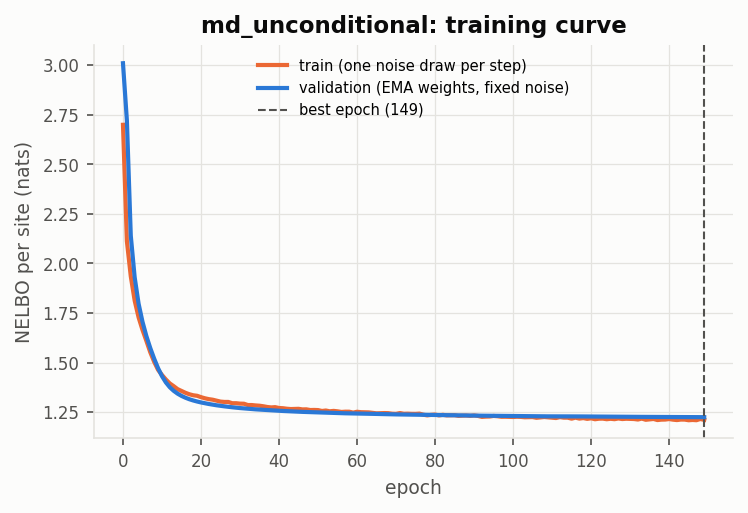
\includegraphics[width=0.55\linewidth]{models/md_unconditional/training_curve.png}
\caption{Training curve of the masked diffusion model (NELBO per site, nats). The two curves overlap; the last
100 epochs gain only 0.025.}
\end{figure}

\subsection{Checkpoints during training}\label{sec:md_checkpoints}
This first run kept its best model only in memory until the end. After it, checkpointing was added to
\texttt{train\_diffusion}, so that a run can be inspected at any time and survive an interruption:
\begin{center}\small
\begin{tabular}{p{0.3\linewidth}p{0.62\linewidth}}
\toprule
file (in \texttt{models/<run>/}) & content and when it is written\\
\midrule
\texttt{model.pt} & the best EMA model so far; rewritten every time the validation NELBO improves (and at the end)\\
\texttt{last.pt} & the complete training state after every epoch: network weights, EMA weights, AdamW moments, learning-rate
schedule, gradient-scaler state, the two random-number generators, history, best value, patience counter\\
\texttt{checkpoints/epoch\_XXX.pt} & a snapshot of the EMA model every \texttt{save\_every} epochs (default 10): the model at
different stages of training, e.g.\ to see how the samples improve\\
\bottomrule
\end{tabular}
\end{center}
\texttt{python scripts/s09\_train\_diffusion.py --config ... --resume} continues from \texttt{last.pt}. Because the optimiser,
schedule, scaler and random-number generators are restored, \textbf{a resumed run is identical to an uninterrupted one}.
\texttt{test\_16\_checkpointing} trains 4 epochs, resumes to 6, and checks that every loss value and every final weight equals
those of a 6-epoch run in one go. It also checks the files and that \texttt{model.pt} equals the returned best model.

\section{Results}\label{sec:md_results}
All comparisons use the held-out test set (1000 sequences per clade) and the same metrics as Part~II.

\subsection{Likelihood bound}
Test NELBO: \textbf{1.219 nats per site} (validation 1.225). This is an upper bound on $-\frac1L\log p_\theta(\bm x)$. The
true value for the data, the entropy per site of the 18-clade mixture, cannot be computed here: it needs the 18 partition
functions. For scale, an independent-site model scores 2.11.

\subsection{The probabilities themselves}
The one-site-masked output $p_\theta(x^i\mid\bm x_{-i})$ was compared, on all 18{,}000 test sequences and 60 sites, with the exact
conditional of the true model of the clade each sequence was drawn from:
\begin{center}\footnotesize
\begin{tabular}{lccc}
\toprule
model & uses the & pseudo-NLL & mean TV to the\\
 & clade label? & per site & true conditional\\
\midrule
true clade models & yes & 0.802 & 0\\
unconditioned Potts $H=128$ & no & 0.949 & 0.154\\
unconditioned Potts $H=256$ & no & 0.945 & 0.152\\
conditioned Potts $H=128$ (true tags) & \textbf{yes} & \textbf{0.872} & \textbf{0.100}\\
conditioned Potts $H=256$ (true tags) & yes & 0.887 & 0.113\\
\textbf{masked diffusion} & \textbf{no} & 0.883 & 0.102\\
\bottomrule
\end{tabular}
\end{center}
Without being told the clade, the diffusion model's conditionals are as close to the truth (TV 0.102) as those of the
best conditioned Potts model \emph{given} the true clade tag (0.100). The network infers the clade from the other 59
residues. Its pseudo-NLL is the second best (0.883 vs 0.872), far ahead of the unconditioned Potts models (0.95).

\begin{figure}[H]
\centering
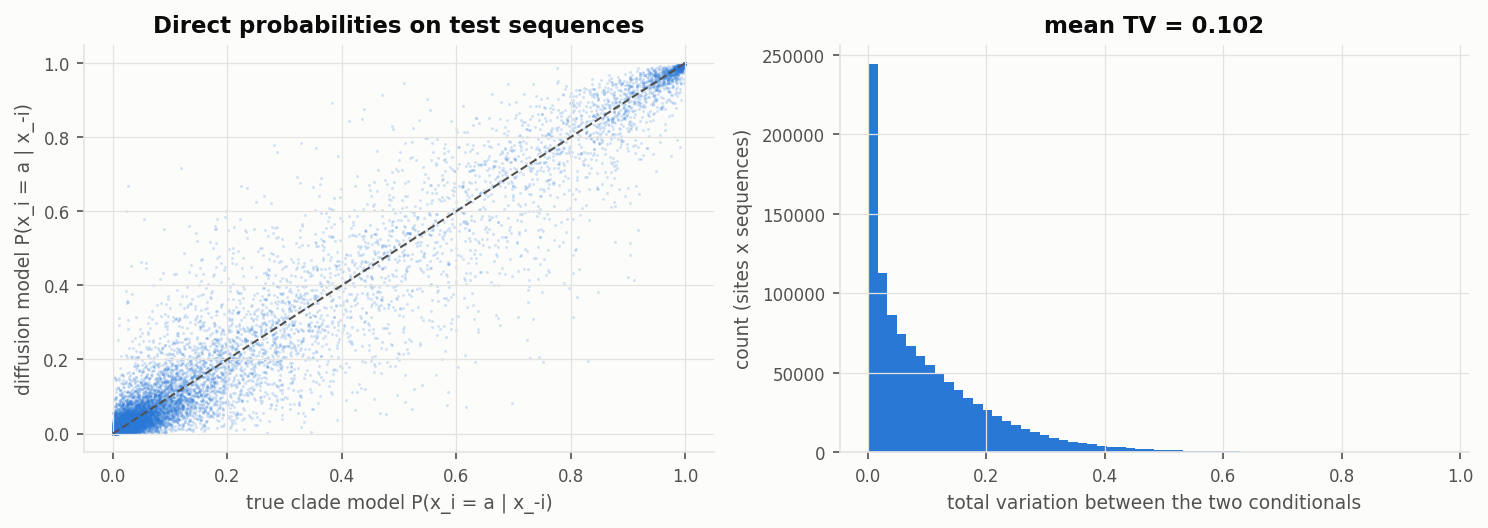
\includegraphics[width=0.85\linewidth]{models/md_unconditional/site_conditionals_vs_truth.png}
\caption{Left: $p_\theta(x^i=a\mid\bm x_{-i})$ vs the true clade conditional (60{,}000 random entries). Right: distribution of the TV
between the two distributions over all sites of all test sequences (median 0.07).}
\end{figure}

\paragraph{Does the network use $t$?} Theory says no (\S\ref{sec:md_optimal}). We fed the same partially masked test sequences
with different $t$ (\texttt{s12}). Changing $t$ from the matching value to anything in $[0.02,1]$ changes the predicted
distributions by a TV of only 0.004--0.03. Two \emph{different} sequences give predictions 0.34--0.56 apart. The network has
learned to (almost) ignore the time input; the small residual grows with the mask fraction.

\subsection{Samples: the sampler matters}
18{,}000 sequences each (as many as the test set):
\begin{center}\footnotesize
\begin{tabular}{lcccccc}
\toprule
sampler & $r_f$ & $r_C$ & slope $C$ & identity & F0/F1/F2 & $\bar d_{NN}$ to train\\
\midrule
$T=15$ steps & 0.999 & 0.987 & 0.81 & 0.197 & 32.3/36.7/30.7\% & 0.425\\
$T=60$ & 1.000 & 0.992 & 0.94 & 0.200 & 33.0/34.1/32.4\% & 0.401\\
$T=240$ & 1.000 & 0.992 & 0.98 & 0.201 & 33.0/32.5/33.7\% & 0.394\\
\textbf{continuous time} & \textbf{1.000} & \textbf{0.992} & \textbf{0.985} & 0.201 & \textbf{33.2/33.0/33.2\%} & 0.393\\
\midrule
oracle (true samples) & 1.000 & 0.994 & 0.99 & 0.197 & 33.1/32.7/33.3\% & 0.378\\
\bottomrule
\end{tabular}
\end{center}
As predicted by \S\ref{sec:md_sampler} and \texttt{test\_13}, few steps weaken the correlations: with $T=15$, about four sites are
revealed per step and drawn independently, and the slope of $C$ drops to 0.81. With $T=60$ it is 0.94, with $T=240$
0.98, and the exact continuous-time sampler reaches 0.985 for the cost of $T=60$. All results below use the
continuous-time sampler.

\begin{figure}[H]
\centering
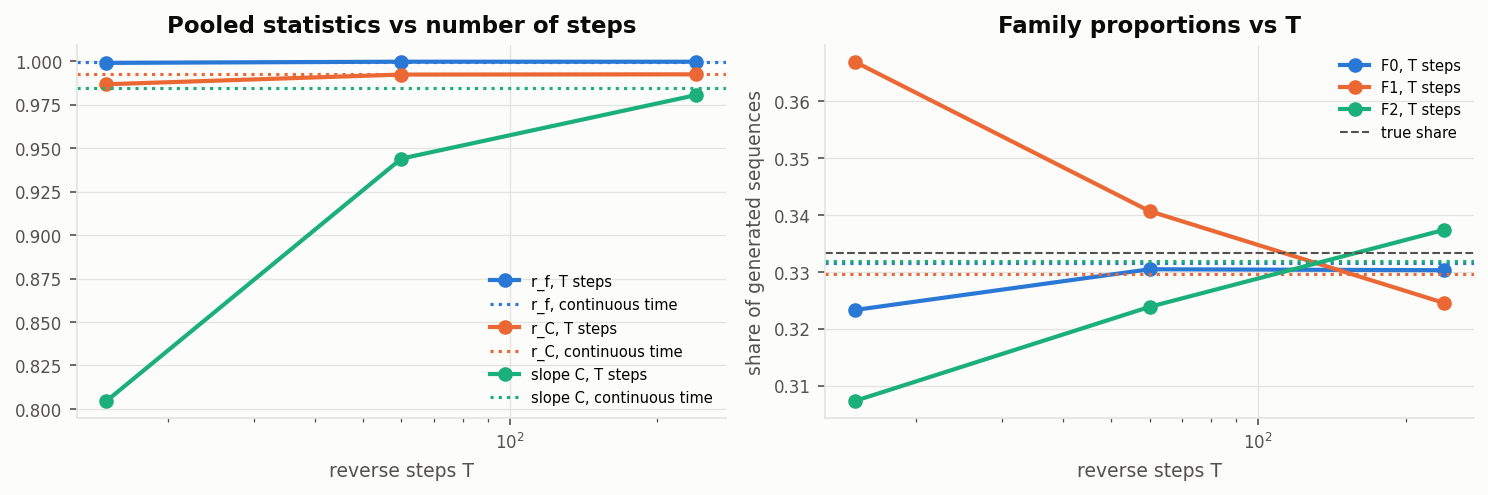
\includegraphics[width=0.9\linewidth]{models/md_unconditional/quality_vs_steps.png}
\caption{Pooled statistics and family proportions vs the number of reverse steps $T$ (dots) and for the continuous-time
sampler (dotted lines).}
\end{figure}

\subsection{Family and clade proportions: fixed}
\begin{center}\footnotesize
\begin{tabular}{lcc}
\toprule
 & family shares F0/F1/F2 & clade shares: TV to 1/18\\
\midrule
oracle & 33.3/33.3/33.3\% & 0.005\\
unconditioned Potts $H=128$ & 21.5/12.8/65.7\% & 0.324\\
unconditioned Potts $H=256$ & 10.7/13.6/75.7\% & 0.424\\
conditioned Potts $H=128$, 18 tags pooled & 33.3/33.3/33.3\% (by construction) & 0.013\\
\textbf{masked diffusion} & \textbf{33.4/33.4/33.2\%} & \textbf{0.011}\\
\bottomrule
\end{tabular}
\end{center}
(Clades are assigned with the pseudo-likelihood classifier of \texttt{s11}: each sequence goes to the true clade model under
which it has the highest pseudo-log-likelihood, which needs no partition function. On the labelled test sequences this
classifier is right for 91.5\% of the clades and 100\% of the families; \texttt{test\_10} checks it on a toy case.)

\textbf{The diffusion model generates the three families, and the 18 clades, in the right proportions}, with no labels,
where the unconditioned Potts models failed badly (\S\ref{sec:res_props}). This is the difference between the two losses.
Pseudo-likelihood never sees the normalisation, so it cannot balance the families. The NELBO bounds the full likelihood, so
a model that gives F2 too much weight pays for it in the loss.

\begin{figure}[H]
\centering
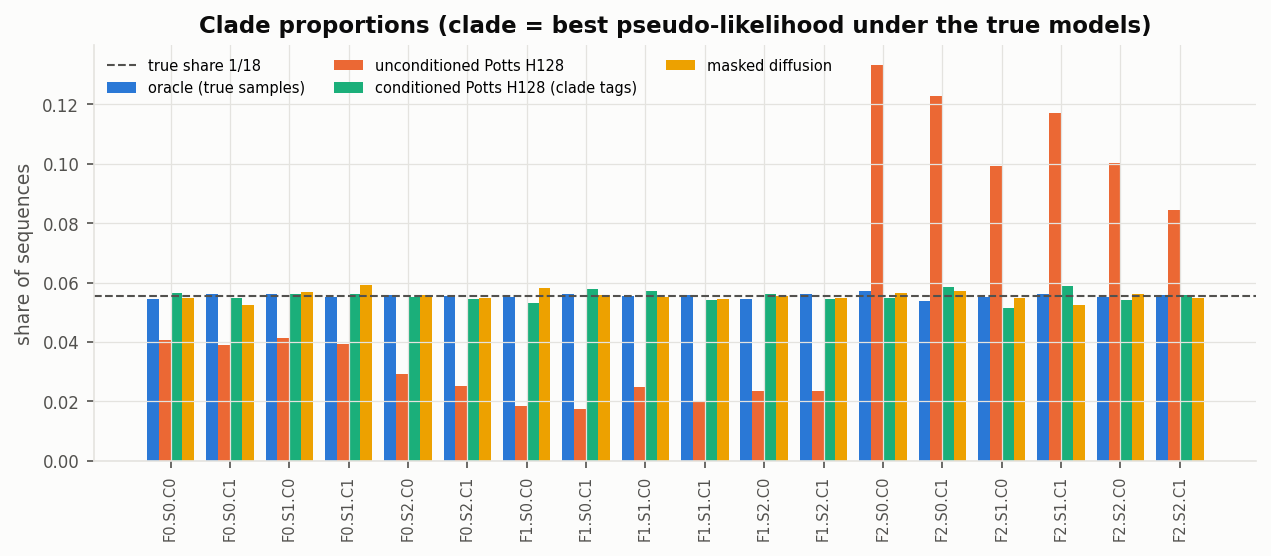
\includegraphics[width=\linewidth]{comparison/clade_proportions.png}
\caption{Share of generated sequences in each clade (assigned by pseudo-likelihood under the true models). Blue: true samples;
orange: unconditioned Potts (F2 clades over-represented); green: conditioned Potts with clade tags; yellow: masked diffusion.}
\end{figure}

\begin{figure}[H]
\centering
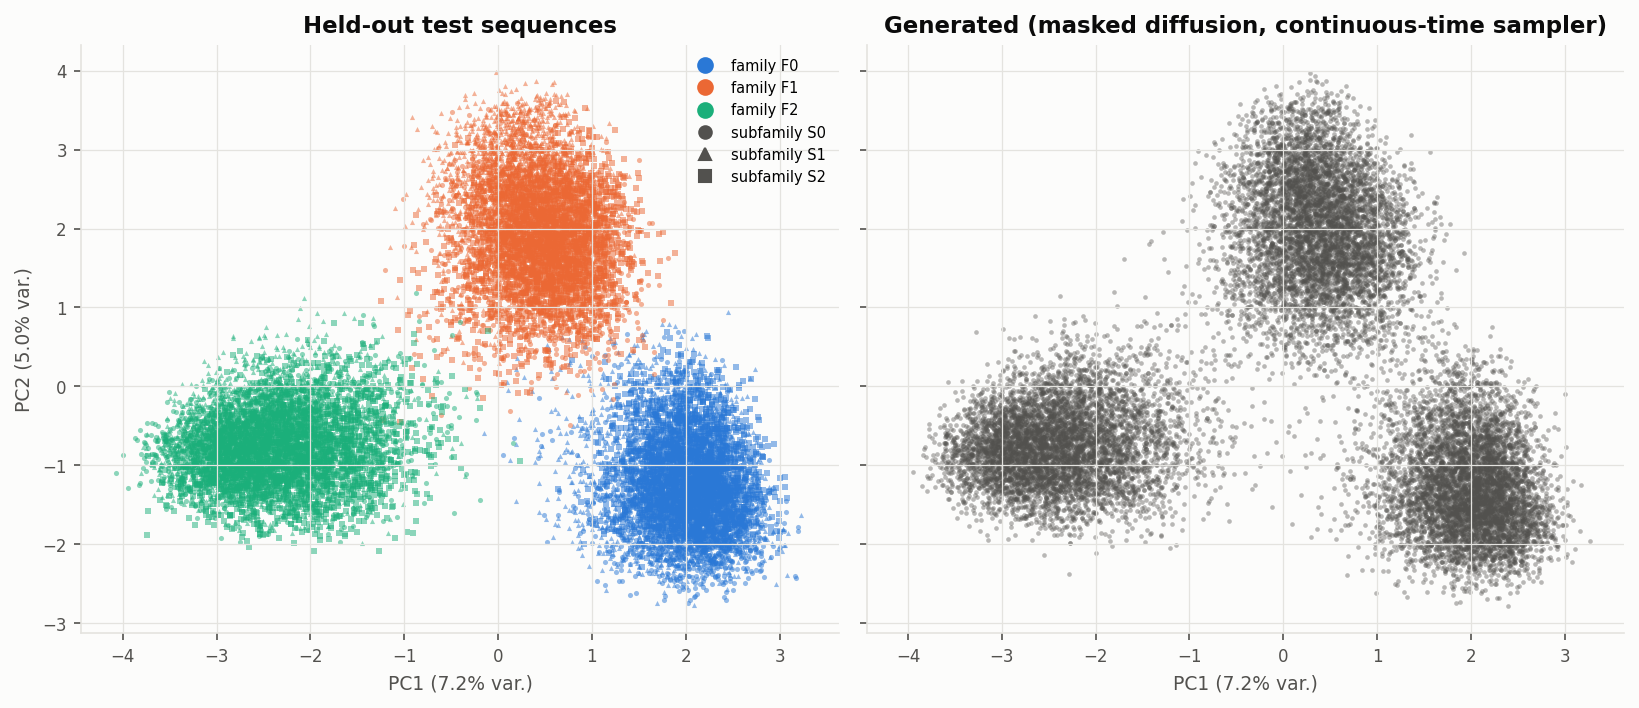
\includegraphics[width=0.85\linewidth]{models/md_unconditional/pca_generated_vs_test.png}
\caption{Test sequences (left) and diffusion samples (right) on the reference PCA: three equally populated families.}
\end{figure}

\subsection{Statistics and distances}
\begin{center}\footnotesize
\begin{tabular}{lcccc}
\toprule
 & unconditioned Potts $H=128$ & \textbf{masked diffusion} & oracle & (test)\\
\midrule
pooled $r_f$ / $r_C$ & 0.940 / 0.895 & \textbf{1.000 / 0.992} & 1.000 / 0.994 & \\
slope of $C$ & 0.70 & \textbf{0.985} & 0.99 & \\
per family: $r_C$ (mean) & 0.83 & \textbf{0.96} & -- & \\
per family: slope of $C$ (mean) & 0.66 & \textbf{0.89} & -- & \\
pairwise $\bar D_{GG}$ & 0.740 & \textbf{0.799} & 0.803 & 0.803\\
Fréchet distance (PCA, pooled) & 2.23 & \textbf{0.005} & 0.001 & \\
mean $d_{NN}$ to train & 0.398 & 0.393 & 0.378 & 0.378\\
copies of training sequences & 0 & 0 & 0 & \\
\bottomrule
\end{tabular}
\end{center}
The pooled statistics are practically those of true samples. Inside each family the correlations are reproduced at
$r_C=0.96$, with a slope of 0.89: slightly too weak, the same direction of error as all previous models but much
smaller. The generated sequences are as diverse as real ones (0.799 vs 0.803), and not copies. They are slightly
\emph{farther} from the training set than real held-out sequences (0.393 vs 0.378, i.e.\ about one site out of 60). This is a
small excess of randomness, consistent with the slightly weak correlations.

\begin{figure}[H]
\centering
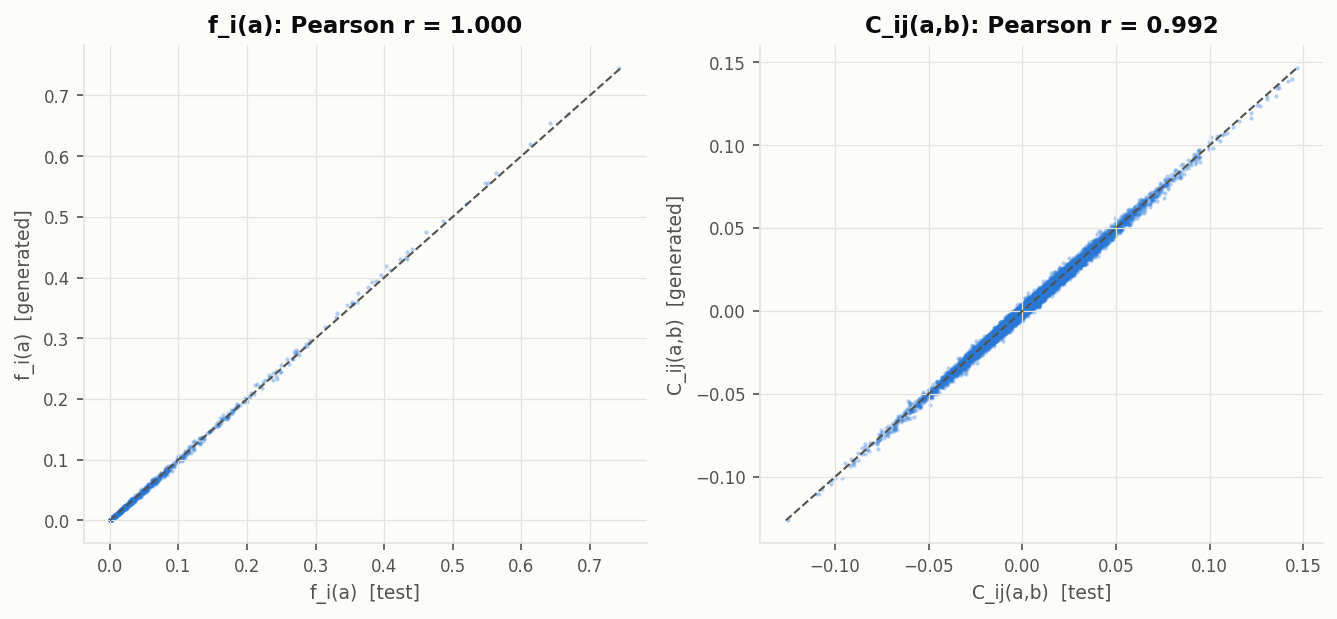
\includegraphics[width=0.49\linewidth]{models/md_unconditional/freq_corr_generated_vs_test.png}\hfill
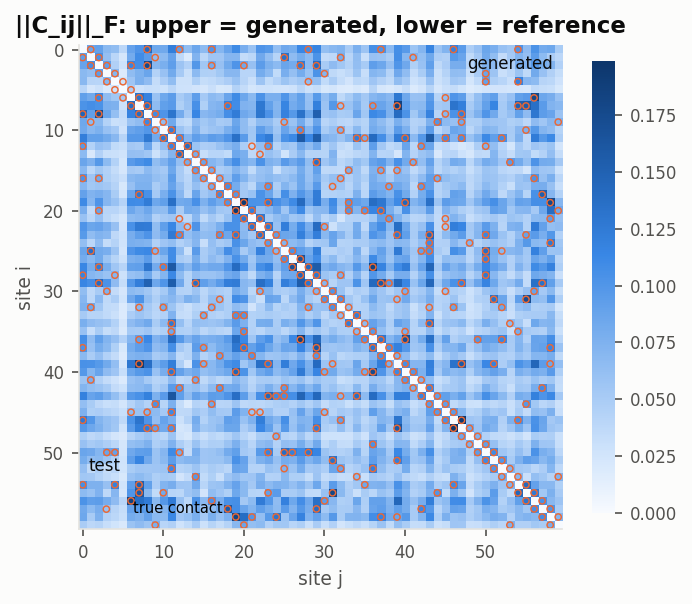
\includegraphics[width=0.4\linewidth]{models/md_unconditional/correlation_strength_test_vs_generated.png}
\caption{Left: site frequencies and connected correlations, diffusion samples vs test. Right: correlation strength map
(lower: test, upper: generated).}
\end{figure}

\begin{figure}[H]
\centering
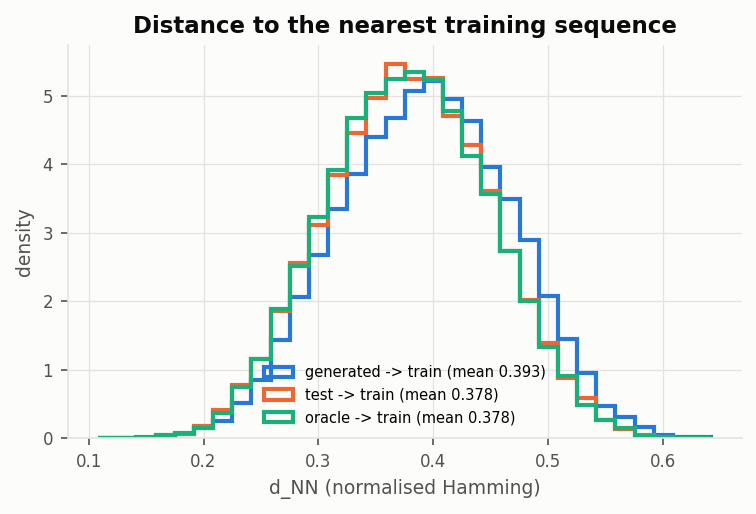
\includegraphics[width=0.49\linewidth]{models/md_unconditional/dist_nn_to_train.png}\hfill
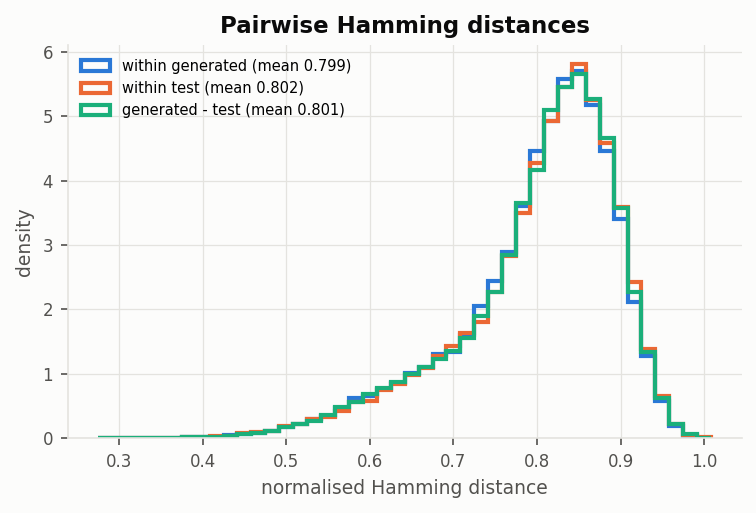
\includegraphics[width=0.49\linewidth]{models/md_unconditional/dist_pairwise.png}
\caption{Distances: nearest training sequence (left) and pairwise Hamming distances (right) for diffusion samples, test and oracle.}
\end{figure}

\subsection{All models at the clade level}
The unconditioned diffusion model can also be judged clade by clade: the generated sequences assigned to clade $c$ are
compared with the test sequences of clade $c$.
\begin{center}\footnotesize
\begin{tabular}{lcccc}
\toprule
 & uses labels & per-clade $r_C$ & per-clade Fréchet & clade shares, TV to 1/18\\
\midrule
oracle & -- & 0.828 & 0.032 & 0.005\\
unconditioned Potts $H=128$ & no & 0.562 & 1.716 & 0.324\\
unconditioned Potts $H=256$ & no & 0.555 & 1.448 & 0.424\\
conditioned Potts $H=128$ & \textbf{yes (tags)} & 0.751 & 0.332 & 0.013\\
\textbf{masked diffusion} & \textbf{no} & \textbf{0.764} & \textbf{0.136} & \textbf{0.011}\\
\bottomrule
\end{tabular}
\end{center}
\begin{figure}[H]
\centering
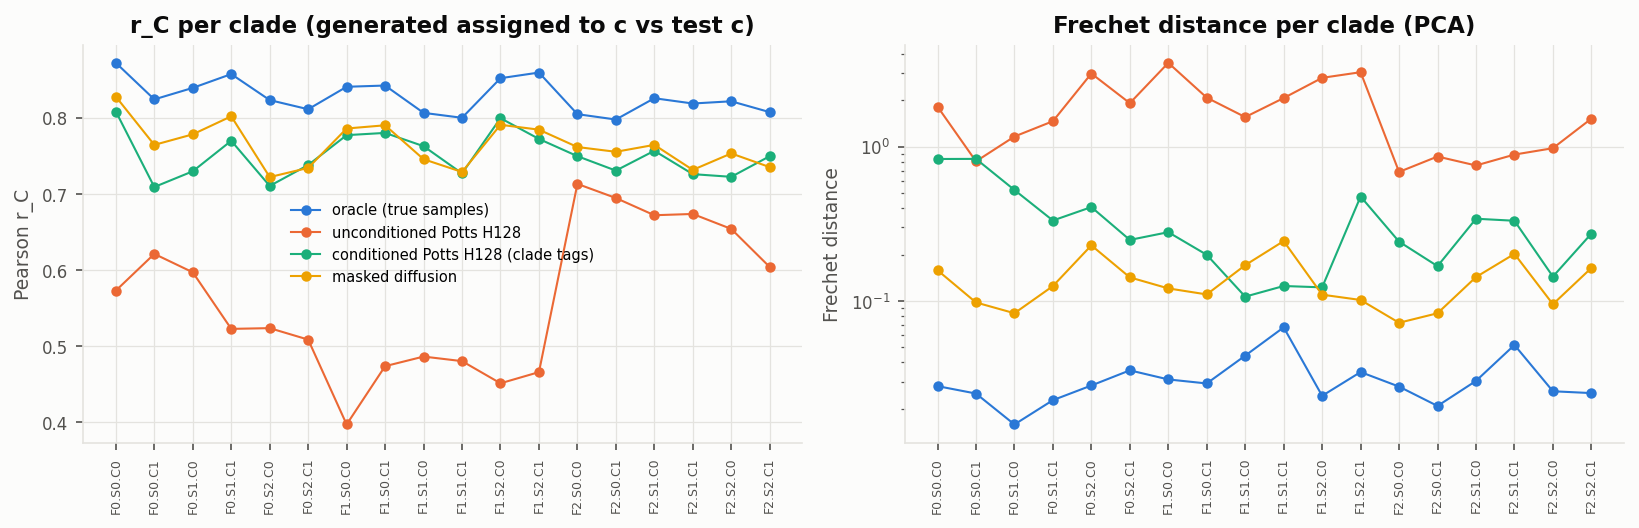
\includegraphics[width=\linewidth]{comparison/per_clade_quality.png}
\caption{Per-clade $r_C$ and Fréchet distance (log scale) of the generated sequences assigned to each clade, for all models.}
\end{figure}

\begin{keybox}{Masked diffusion: summary}
\begin{itemize}[nosep]
\item[+] \textbf{Right global weights}: families 33/33/33\%, clades within 0.011 of uniform, without labels. Training on a
      likelihood bound fixes the main failure of the pseudo-likelihood models.
\item[+] \textbf{Best generator so far}: pooled $r_C=0.992$ (oracle 0.994), Fréchet 0.005 (oracle 0.001); per clade it matches or beats
      the conditioned Potts model that is \emph{given} the clade tag ($r_C$ 0.764 vs 0.751, Fréchet 0.14 vs 0.33).
\item[+] \textbf{Correct probabilities}: its conditionals are as close to the true clade conditionals (TV 0.10) as those of the
      tag-conditioned Potts model; it infers the clade from the sequence.
\item[+] No memorisation; diversity equal to real sequences.
\item[--] Correlations inside a family are still $\approx10\%$ too weak (slope 0.89), and the samples are about one site more
      ``random'' than real sequences. Training had not fully converged (best epoch $=$ last epoch).
\item[--] It gives no interpretable $J$; the price of not assuming a Potts form. It is also 2--9$\times$ larger (4.8\,M parameters vs 0.5--2.1\,M)
      and 10--100$\times$ more expensive to train than the factored-attention models (4\,h vs 2--23\,min).
\item[!] The sampler matters: few reverse steps destroy correlations; use the exact continuous-time sampler.
\end{itemize}
\end{keybox}
